\chapter{\RU{Указатели}\EN{Pointers}}
\index{\CLanguageElements!\Pointers}
\label{label_pointers}

\newcommand{\ttf}{\TT{f1()}}

\RU{Указатели также часто используются для возврата значений из функции (вспомните случай
со \scanf{}~(\ref{label_scanf}))}
\EN{Pointers are often used to return values from function (recall \scanf case~(\ref{label_scanf}))}.
\RU{Например, когда функции нужно вернуть сразу два значения}
\EN{For example, when function should return two values}.

\section{\RU{Пример с глобальными переменными}\EN{Global variables example}}

\lstinputlisting{patterns/061_pointers/global.c}

\RU{Это компилируется в}\EN{This compiling into}:

\lstinputlisting[caption=\Optimizing MSVC 2010 (/Ox /Ob0)]{patterns/061_pointers/global.asm}

\index{\olly}
\RU{Посмотрим это в}\EN{Let's see this in} \olly: \figref{fig:pointers_olly_global_1}.
\RU{В начале адреса обоих глобальных переменных передаются в}\EN{At first, global
variables addresses are passed into} \ttf.
\RU{Можно нажать}\EN{We can click} ``Follow in dump'' \RU{на элементе стека и в окне слева 
увидим место в сегменте данных выделенных для двух переменных}\EN{on the stack element, and we will see 
a place in data segment allocated for two variables}.
\RU{Эти переменные обнулены, потому что, по стандарту, неинициализированные данные (\ac{BSS}) 
обнуляются перед началом исполнения}
\EN{These variables are cleared, because non-initialized data (\ac{BSS}) are cleared before
execution begin}.
\RU{И они находятся в сегменте данных, о чем можно удостовериться нажав}
\EN{They are residing in data segment, we can be sure it is so, by pressing} Alt-M \RU{и увидев карту
памяти}\EN{and seeing memory map}: \figref{fig:pointers_olly_global_5}.

\RU{Трассируем}\EN{Let's trace} (F7) \RU{до начала исполнения}\EN{until execution of} \ttf 
\figref{fig:pointers_olly_global_2}.
\RU{В стеке видны и значения}\EN{Two values are seen in the stack} $456$ (\TT{0x1C8}) \AndENRU 
$123$ (\TT{0x7B}), \RU{а также адреса двух глобальных переменных}\EN{and two global variables addresses
as well}.

\RU{Трассируем до конца}\EN{Let's trace until the end of} \ttf.
\RU{Мы видим в окне слева, как результаты вычисления появились в глобальных переменных}
\EN{At the window at left we see how calculation results are appeared in the gloval variables} 
\figref{fig:pointers_olly_global_3}.

\RU{Теперь из глобальных переменных значения загружаются в регистры для передачи в}
\EN{Now values of global variables are loaded into registers for passing into} \printf:
\figref{fig:pointers_olly_global_4}.

\begin{figure}[H]
\centering
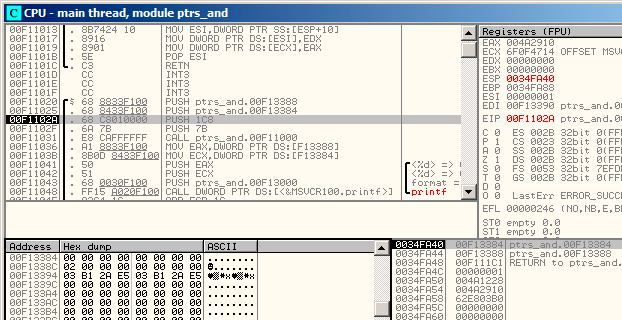
\includegraphics[scale=\FigScale]{patterns/061_pointers/olly_global1.png}
\caption{\olly: \RU{передаются адреса двух глобальных переменных в}
\EN{global variables addresses are passing into} \ttf}
\label{fig:pointers_olly_global_1}
\end{figure}

\begin{figure}[H]
\centering
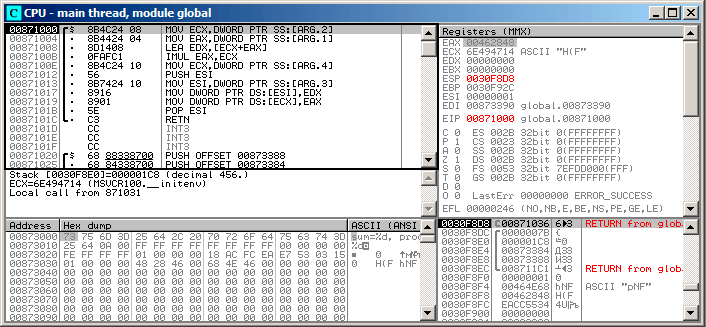
\includegraphics[scale=\FigScale]{patterns/061_pointers/olly_global2.png}
\caption{\olly: \RU{начало работы \ttf}\EN{\ttf is started}}
\label{fig:pointers_olly_global_2}
\end{figure}

\begin{figure}[H]
\centering
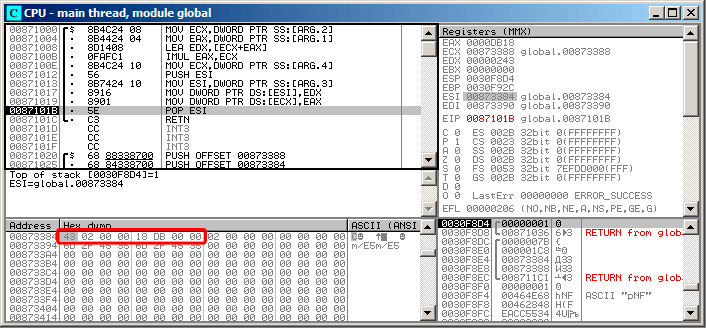
\includegraphics[scale=\FigScale]{patterns/061_pointers/olly_global3.png}
\caption{\olly: \ttf \RU{заканчивает работу}\EN{finishes}}
\label{fig:pointers_olly_global_3}
\end{figure}

\begin{figure}[H]
\centering
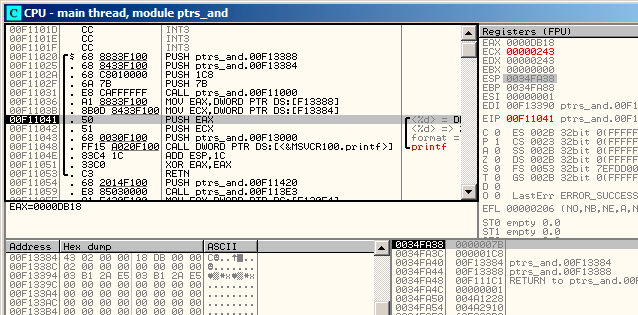
\includegraphics[scale=\FigScale]{patterns/061_pointers/olly_global4.png}
\caption{\olly: \RU{адреса глобальных переменных передаются в}
\EN{global variables addresses are passed into} \printf}
\label{fig:pointers_olly_global_4}
\end{figure}

\begin{figure}[H]
\centering
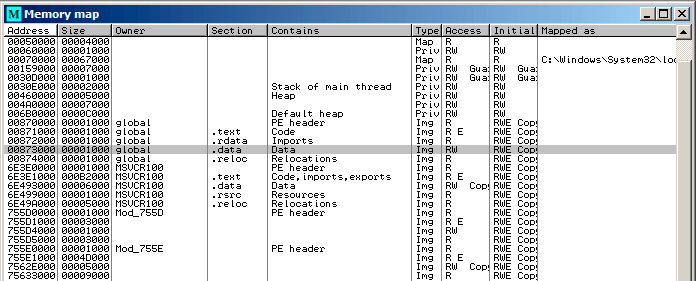
\includegraphics[scale=\FigScale]{patterns/061_pointers/olly_global5.png}
\caption{\olly: \RU{карта памяти}\EN{memory map}}
\label{fig:pointers_olly_global_5}
\end{figure}

\section{\RU{Пример с локальными переменными}\EN{Local variables example}}

\RU{Немного переделаем пример}\EN{Let's rework our example slightly}:

\lstinputlisting[caption=\RU{теперь переменные локальные}
\EN{now variables are local}]{patterns/061_pointers/local_\LANG.c}

\RU{Код ф-ции }\ttf \RU{не изменится}\EN{function code will not changed}.
\RU{Изменится только \main}\EN{Only \main code will}:

\lstinputlisting[caption=\Optimizing MSVC 2010 (/Ox /Ob0)]{patterns/061_pointers/local.asm}

\newcommand{\PtrsAddresses}{\TT{0x35FCF4} \AndENRU \TT{0x35FCF8}\xspace}

\RU{Снова посмотрим в}\EN{Let's again take a look into} \olly.
\RU{Адреса локальных переменных в стеке это}\EN{Local variable addresses in the stack are} \PtrsAddresses.
\RU{Видно как они заталкиваются в стек}\EN{We see how these are pushed into the stack}: 
\figref{fig:pointers_olly_stk_1}.

\RU{Начало работы \ttf}\EN{\ttf is started}.
\RU{В стеке по адресам}\EN{Random garbage are at} \PtrsAddresses \RU{пока находится случайный мусор}
\EN{so far} \figref{fig:pointers_olly_stk_2}.

\RU{Конец работы \ttf}\EN{\ttf finished}.
\RU{В стеке по адресам \PtrsAddresses теперь значения \TT{0xDB18} \AndENRU \TT{0x243}, 
это результаты работы \ttf}
\EN{There are \TT{0xDB18} \AndENRU \TT{0x243} now at \PtrsAddresses addresses, these values are
\ttf function result}.

\begin{figure}[H]
\centering
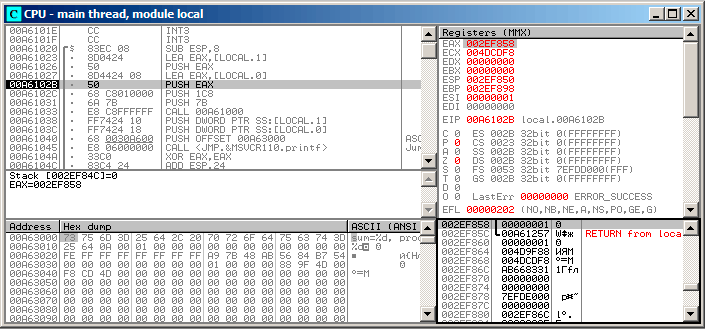
\includegraphics[scale=\FigScale]{patterns/061_pointers/olly_stk1.png}
\caption{\olly: \RU{адреса локальных переменных заталкиваются в стек}\EN{addresses of local variables are
pushed into the stack}}
\label{fig:pointers_olly_stk_1}
\end{figure}

\begin{figure}[H]
\centering
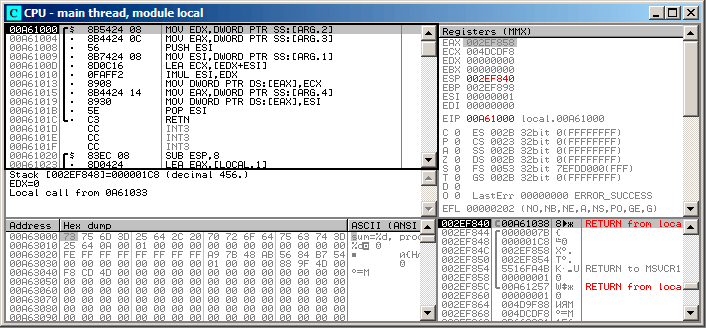
\includegraphics[scale=\FigScale]{patterns/061_pointers/olly_stk2.png}
\caption{\olly: \ttf \RU{начинает работу}\EN{starting}}
\label{fig:pointers_olly_stk_2}
\end{figure}

\begin{figure}[H]
\centering
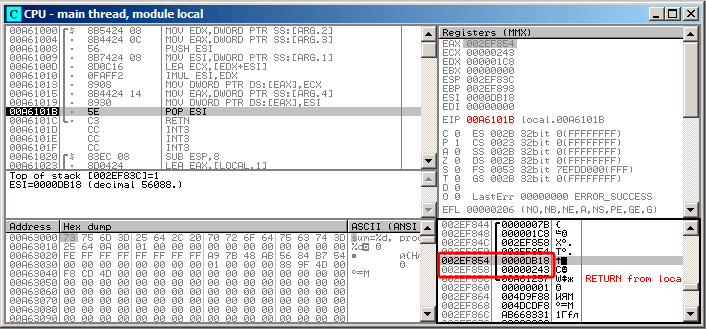
\includegraphics[scale=\FigScale]{patterns/061_pointers/olly_stk3.png}
\caption{\olly: \ttf \RU{заканчивает работу}\EN{finished}}
\label{fig:pointers_olly_stk_3}
\end{figure}

\section{\Conclusion{}}

\RU{\ttf может одинаково хорошо возвращать результаты работы в любые места памяти, 
находящиеся где угодно}\EN{\ttf can return results to any place in memory, located anywhere}.
\RU{В этом суть и удобство указателей}\EN{This is essence and usefulness of pointers}.

\RU{Кстати,}\EN{By the way, \Cpp} \IT{references} \RU{в \Cpp работают точно так же}\EN{works just in the
same way}. \RU{Читайте больше об этом}\EN{Read more about them}: (\ref{cpp_references}).

